%!TEX root = mieic.tex
\chapter{Solução Implementada} \label{chap:sol}

\section*{}

Neste capítulo é descrita de forma pormenorizada a solução implementada de modo a responder aos desafios colocados na introdução, cumprindo assim os objetivos propostos.
Inicialmente é caracterizada a arquitetura definida, fazendo referência aos diferentes componentes que constituem o produto final. Posteriormente são referidas de uma forma breve as tecnologias envolvidas no seu desenvolvimento.
Por último é especificada a \textit{framework} desenvolvida e o exemplo implementado.

\section{Visão Geral} \label{sec:geral}

Tal como foi referido na definição dos objetivos, era esperado o desenvolvimento e validação de uma arquitetura que permitisse uma interação baseada na manipulação direta, através de um dispositivo móvel, facilitando a criação de aplicações para ecrãs públicos.  
Na solução encontrada, de uma maneira global, é possível diferenciar três diferentes componentes, sendo eles o servidor, desenvolvido em \textit{node.js}, a aplicação, que irá correr no servidor criado comunicando com este através de \textit{web sockets} e ainda o utilizador final, aqui identificado como cliente.

A figura~\ref{fig:componentes} apresenta, de uma forma simples, os componentes acima descritos.

\begin{figure}[ht]
\centering
\includegraphics[scale=0.45]{components.pdf}
\caption[Componentes] {Componentes constituintes da solução desenvolvida}
\label{fig:componentes}
\end{figure}

Na figura ~\ref{fig:sequencia} é representado um diagrama de sequência mostrando as diferentes interações entre os componentes constituintes do sistema implementado. Inicialmente terá de existir um pedido por parte de um ecrã para aceder à aplicação, neste momento a aplicação comunica com o servidor e a partir daqui está preparada para pedidos de possíveis utilizadores. Um utilizador, ao querer interagir com a aplicação está a enviar um pedido para esta, que por sua vez avisa o servidor e este é responsável por mostrar no dispositivo o \textit{widget} da aplicação. Neste momento o \textit{widget} liga-se ao servidor e após ocorrer a ligação procede-se à troca de ``mensagens'' que permitem ao utilizador definir o seu nome. Quando o cliente tiver o nome definido pode usufruir do \textit{widgets} disponíveis, realizando-se a comunicação para o servidor, que por sua vez envia para a aplicação.

\begin{figure}[ht]
\centering
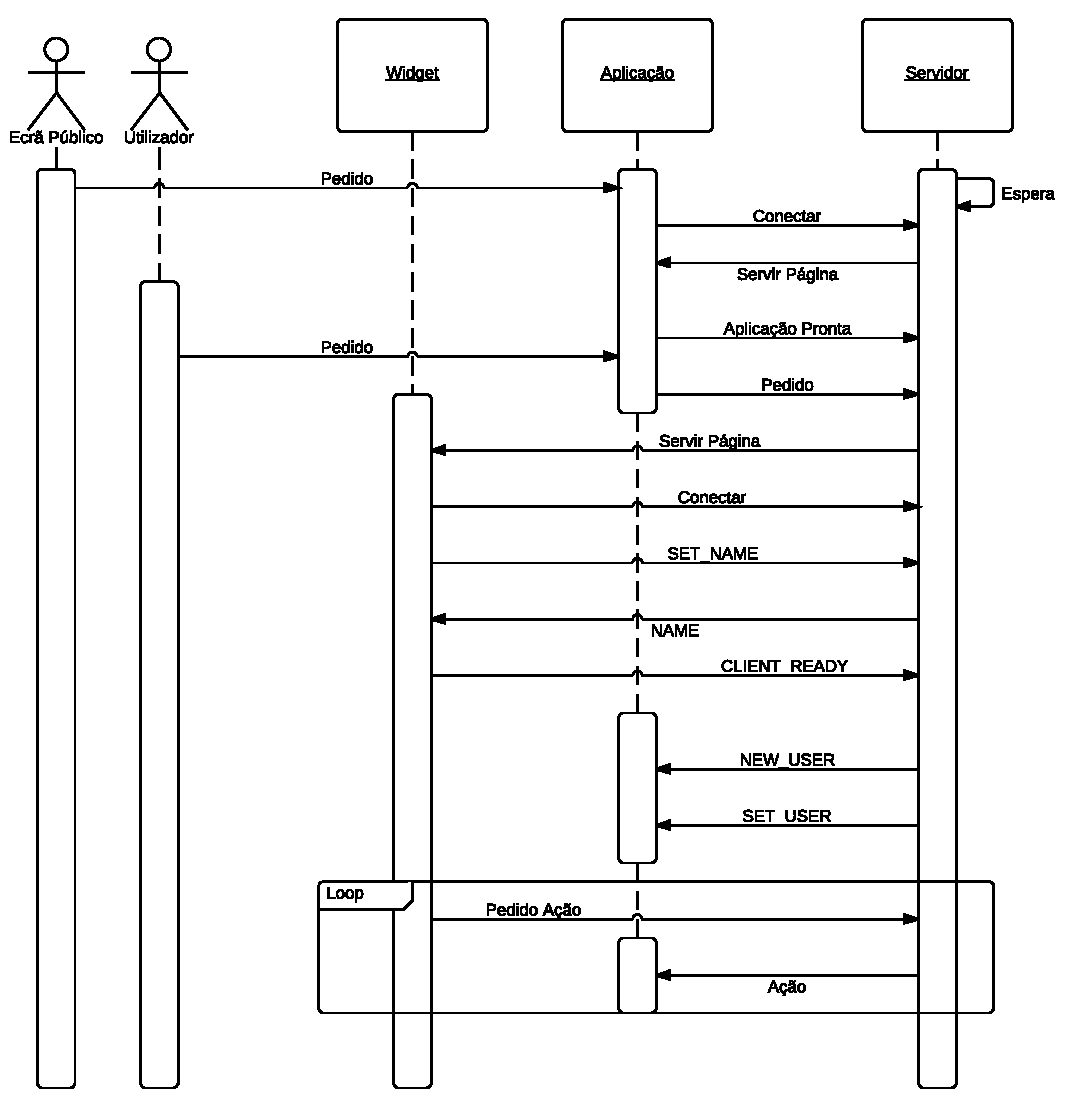
\includegraphics[scale=0.63]{Sequence.pdf}
\caption[Diagrama de Sequência] {Diagrama de Sequência}
\label{fig:sequencia}
\end{figure}


\section{Tecnologias Usadas} \label{sec:tec}

Ao longo da implementação houve necessidade de optar por diversas tecnologias para que fosse possível alcançar o objetivo desejado, \textit{Node.js} foi usado para a implementação do servidor e \textit{web sockets} e \textit{socket.io} para facilitar a comunicação entre os diversos componentes. Foi também usada a \textit{framework} \textit{Prototype} que permite a manipulação de classes em \textit{JavaScript}, e uma biblioteca, \textit{Swipeable} que dá resposta a eventos \textit{swipe} facilitando a utilização.

\begin{itemize}

\item \textbf{Node.js}


\textit{Node.js} é uma plataforma construída para facilitar o desenvolvimento de aplicações de alta escalabilidade em tempo real, com base no interpretador \textit{Javascript V8} da \textit{Google}, que antes da execução compila \textit{JavaScript} em código máquina, melhorando consideravelmente o tempo de execução. Deste modo \textit{Node} permite a construção de aplicações rápidas e altamente concorrentes.

Segundo Michael Abernethy ~\cite{Abernethy2011} node altera a noção de como um servidor deve funcionar, referindo que o seu objetivo é permitir que um programador construa aplicações com grande escalabilidade e que o código desenvolvido suporte milhares de ligações simultâneas numa só máquina. 

\textit{Node.js} opera uma \textit{thread} simples, não bloqueia as chamadas de entrada e saída, permitindo o suporte das diversas ligações ~\ref{fig:node}.

\begin{figure}[ht]
\centering
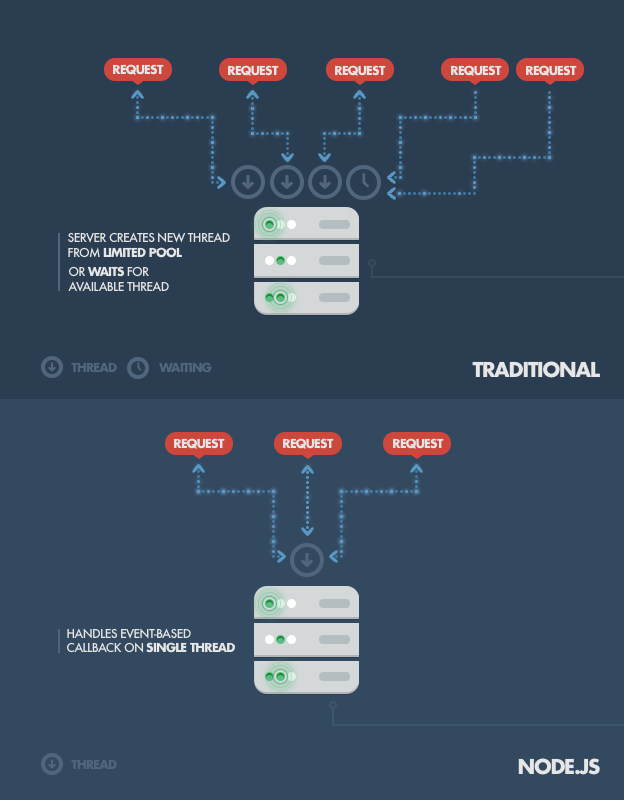
\includegraphics[scale=0.4]{node.png}
\caption[\textit{Node.js}] {Diferença entre técnicas tradicionais de servidores e \textit{Node.js}\protect\footnotemark}
\label{fig:node}
\end{figure}

\footnotetext{http://www.toptal.com/nodejs/why-the-hell-would-i-use-node-js}

\item \textbf{Web Sockets}

De forma a permitir a comunicação do utilizador, lado do cliente, com o servidor criado foram usados web sockets. Estes foram desenvolvidos para serem implementados em em aplicações ou servidores web, usando um protocolo independente baseado em TCP.

O protocolo \textit{websocket} encontra-se normalizado, o que significa que é seguida uma norma no envio de informação entre o servidor e o \textit{browser} sem que haja uma solicitação por parte do cliente o que possibilita uma maior interação entre estes, facilitando a criação de aplicações em tempo real. É deste modo criada uma ligação bi-direcional entre o \textit{browser} e o servidor, pois a conexão é mantida aberta enquanto as mensagens são encaminhadas de um lado para o outro.


\item \textbf{Socket.io}

\textit{Socket.io} é descrita como uma biblioteca \textit{JavaScript} usada no desenvolvimento de aplicações web. Esta é composta por 2 partes, uma biblioteca para o lado do cliente, que corre no \textit{browser}, e outra para o lado do servidor, que para já terá de ser implementado em \textit{node.js}, daí este estar acima referido como uma das tecnologias usadas. Quer o lado do cliente quer o do servidor apresentam \textit{API’s} idênticas. 
Usa, principalmente como protocolo, \textit{websockets}, também escolhido como tecnologia usada no desenvolvimento desta solução, contudo, se necessário, podem ser utilizados outros, como por exemplo \textit{Adobe Flash sockets, JSONP polling}, e \textit{AJAX long polling}. 
A sua escolha aliada a \textit{websockets} fornece bastante recursos, como a transmissão para múltiplos sockets, armazenamento de informação associada a cada cliente e ainda ``inputs/outputs'' assíncronos. 

\item \textbf{Prototype}

\textit{Prototype} é uma \textit{framework} em \textit{JavaScript} que fornece algumas funções para o desenvolvimento de aplicações em \textit{JavaScript}. As suas funcionalidades variam entre pequenos atalhos de programação e principais funções para lidar com \textit{XMLHttpRequest}.

Esta \textit{framework} fornece ainda uma biblioteca com funções que suporta classes e objetos baseados em classes, algo que não é possível em \textit{JavaScript}.

\item \textbf{Swipeable}

\textit{Swipeable} trata-se de uma biblioteca que permite obter resposta a eventos \textit{swipe} realizados num dispositivo \textit{touch}, sendo uma abstração do \textit{touchstart}, \textit{touchmove} e \textit{touchend}. 
Foi incluída no ficheiro \textit{widget.js} de para possibilitar o desenvolvimento e correto funcionamento do controlo através de \textit{swipe}.

\end{itemize}

Para além das tecnologias acima definidas todo o projeto foi realizado recorrendo a JavaScript, HTML e CSS. 


\section{\textit{Framework} Desenvolvida} \label{sec:framework}

Um dos principais objetivos centrava-se no desenvolvimento de uma \textit{framework} que facilitasse o desenvolvimento de aplicações para ecrãs públicos, que permitissem a manipulação direta por parte dos utilizadores, deste modo, surge a criação de uma pequena API que permite a construção e utilização de três diferentes tipos de controlo. 
Na figura~\ref{fig:classes} é representada a estrutura usada, mostrando as classes constituintes, respetivos atributos e métodos e ainda a relação entre as classes.

\begin{figure}[ht]
\centering
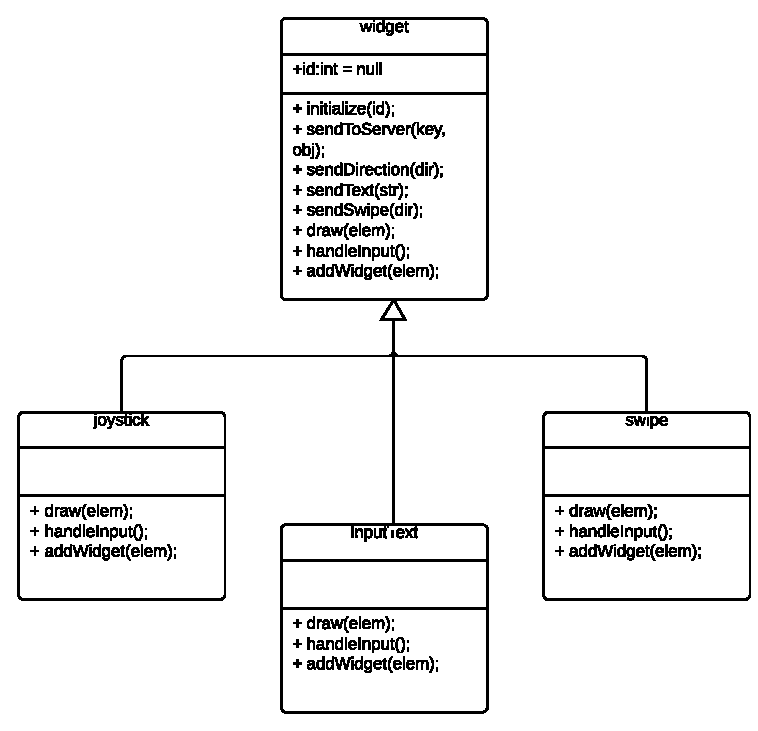
\includegraphics[scale=0.5]{classes.pdf}
\caption[\textit{classes}] {Diagrama de classes}
\label{fig:classes}
\end{figure}

A classe \textit{Widget} representa uma abstração dos controlos possíveis, sendo a classe \textit{Joystick}, \textit{Swipe} e \textit{inputText} instâncias desta. Uma vez que se trata de uma relação de herança, quer os atributos, quer os métodos da super classe são herdados pelas respetivas subclasses, permitindo a sua utilização.

\subsection{Funcionalidades}

	Com o objetivo de facilitar a criação de aplicações para ecrãs públicos, foi desenvolvida uma pequena API, com um conjunto de funcionalidades que permitem a um programador o seu uso na criação de diferentes controlos de acordo.

	A classe \textit{Widget}, já definida anteriormente, apresenta alguns métodos, próprios que são usados nas subclasses permitindo a comunicação com o servidor, tabela ~\ref{table:widget_met}.

	\begin{table}[ht]
 	\renewcommand{\arraystretch}{1.5}
	\centering

	\begin{tabular}{ p{2cm}|p{2cm}|p{10cm}  }
	\multicolumn{1}{c}{\textbf{Métodos}} & \multicolumn{1}{c}{\textbf{Parâmetros}} & \multicolumn{1}{c}{\textbf{Descrição}} \\
	\hline
	\multicolumn{1}{c}{initialize} & \multicolumn{1}{c}{id} &Método responsável por inicializar o \textit{widget} \\
	\hline
	\multicolumn{1}{c}{sendToServer} & \multicolumn{1}{c}{} &Método responsável por realizar a comunicação com o servidor \\
	\hline
	\multicolumn{1}{c}{sendDirection} & \multicolumn{1}{c}{dir} &Método que usa o método \textit{sendToServer} para enviar a direção, dir, obtida pelo \textit{widget joystick} \\
	\hline
	\multicolumn{1}{c}{sendText} & \multicolumn{1}{c}{str} &Método que usa o método \textit{sendToServer} para enviar texto, str, obtida pelo \textit{widget}  \\
	\hline
	\multicolumn{1}{c}{sendSwipe} & \multicolumn{1}{c}{dir} &Método que usa o método \textit{sendToServer} para enviar a direção, dir, obtida pelo \textit{widget swipe}  \\
	\hline
	\end{tabular}
	\caption{Métodos da classe \textit{Widget}}
	\label{table:widget_met}
	\end{table}
	
	Os controlos referidos dizem respeito aos diferentes tipos de controlo que estão disponíveis para ser usados em qualquer aplicação, e na solução apresentada disponibilizam os métodos presentes na tabela ~\ref{table:metodos}:
	
 	\begin{table}[ht]
 	\renewcommand{\arraystretch}{1.5}
	\centering

	\begin{tabular}{ p{2cm}|p{2cm}|p{10cm}  }
	\multicolumn{1}{c}{\textbf{Métodos}} & \multicolumn{1}{c}{\textbf{Parâmetros}} & \multicolumn{1}{c}{\textbf{Descrição}} \\
	\hline
	\multicolumn{1}{c}{draw} & \multicolumn{1}{c}{elem} &Método responsável por desenhar o widget correspondente no elemento (elem) da página html apresentada no dispositivo \\
	\hline
	\multicolumn{1}{c}{handleInput} & \multicolumn{1}{c}{} &Método responsável por atribuir eventos aos widgets \\
	\hline
	\multicolumn{1}{c}{addWidget} & \multicolumn{1}{c}{elem} &Método responsável por adicionar o widget à barra de widgets disponíveis no elemento, elem, da página html \\
	\hline
	\multicolumn{1}{c}{setOptions} & \multicolumn{1}{c}{options} &Método que permite ao programador alterar o conteúdo do que é enviado do widget para a aplicação  \\
	\hline
	\end{tabular}
	\caption{Métodos disponíveis em cada um dos widget}
	\label{table:metodos}
	\end{table}


Para além dos métodos acima descritos, que constituem as opções disponíveis para a instância de cada tipo de \textit{widget}, o programador tem disponíveis outros dois, que podem ser vistos na tabela ~\ref{table:metodos_g}:

	\begin{table}[ht]
 	\renewcommand{\arraystretch}{1.5}
	\centering

	\begin{tabular}{ p{2cm}|p{2cm}|p{10cm}  }
	\multicolumn{1}{c}{\textbf{Método}} & \multicolumn{1}{c}{\textbf{Parâmetros}} & \multicolumn{1}{c}{\textbf{Descrição}} \\
	\hline
	\multicolumn{1}{c}{start} & \multicolumn{1}{c}{url, options} &Método para inicializar o widgets, responsável por efetuar a ligação com o servidor \\
	\hline
	\multicolumn{1}{c}{drawBar} & \multicolumn{1}{c}{elem} &Método por desenhar, no elemento, elem, da página html, a barra que mostra ao utilizador os widgets que tem disponíveis \\
	\hline
	\end{tabular}
	\caption{Métodos Gerais}
	\label{table:metodos_g}
	\end{table}


\subsection{Controlos Definidos}

	A API desenvolvida apresenta três diferentes tipos de controlos, como mostra a figura~\ref{fig:widgets}, que o programador terá à sua disposição para implementar, de acordo com aplicação desenvolvida. Neste momento existem como possíveis opções, o \textit{joystick}, o \textit{swipe} e ainda outro composto por uma caixa de introdução de texto.

	\begin{itemize}

	\item \textbf{Joystick}

		Controlo composto pelas quatro setas tradicionais, esquerda, direita, cima e baixo, que pode ser utilizado em qualquer aplicação que exija uma movimentação.

	\item \textbf{Swipe}

		Controlo que usa as propriedade \textit{touch} do dispositivo para controlar a aplicação, definido apenas para reconhecer uma direção, contudo pode ser alterado.

	\item \textbf{InputText}

		Controlo que permite ao utilizador a interação com aplicações que exijam a introdução de texto.

	\end{itemize}

	\begin{figure}[ht]
	  \centering
	  \leavevmode
	  \begin{subfigure}{.33\textwidth}
	    \centering
	    
\includegraphics[width=.8\linewidth]{joystick}
	    \caption{\textit{Widget Joysitck}}
	    \label{fig:joystick}
	  \end{subfigure}%
	  \begin{subfigure}{.33\textwidth}
	    \centering
	    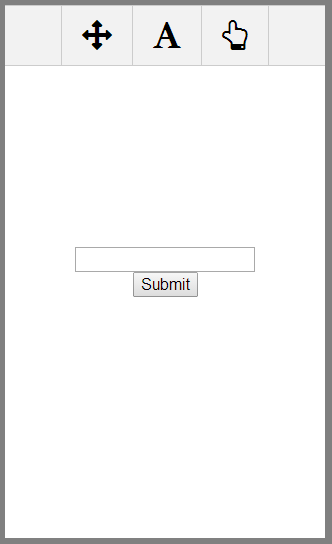
\includegraphics[width=.8\linewidth]{text}
	    \caption{\textit{Widget InputText}}
	    \label{fig:inputext}
	  \end{subfigure}%
	   \begin{subfigure}{.33\textwidth}
	    \centering
	    
\includegraphics[width=.8\linewidth]{swipe}
	    \caption{\textit{Widget Swipe}}
	    \label{fig:swipe}
	  \end{subfigure}
	  \caption{Diferentes Tipos de Controlo Disponíveis}
	  \label{fig:widgets}
	\end{figure}

\subsection{Utilização}

	O desenvolvimento da \textit{framework} apresentada tinha como objetivo auxiliar na criação de controlos para aplicações com as quais fosse possível interagir em ambiente público com um dispositivo móvel.

	Um programador que pretenda usufruir das suas funcionalidades deverá:

	\begin{itemize}
		\item Criar um documento html com o nome \textit{widget.html} e a estrutura apresentada na figura ~\ref{fig:html_struct}
		\item Incluir no ficheiro as seguintes bibliotecas:
			\begin{itemize}
			\item prototype.js 
			\item swipeable.js
			\item socket.io
			\end{itemize}
		\item Incluir no mesmo ficheiro um script onde são chamadas as funções da API.
	\end{itemize}

	\begin{figure}[ht]
		\centering
		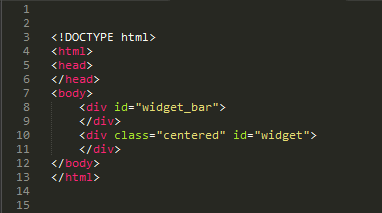
\includegraphics[scale=1]{html}
		\caption[Estrutura html] {Estrutura para criação de \textit{widgets}}
		\label{fig:html_struct}
	\end{figure}

	Apesar de haver liberdade nas escolha dos widgets a implementar, independentemente disto, o método \textit{start(url,options)} tem obrigatoriamente de ser chamado antes da criação dos \textit{widgets} pretendidos. 


	
\section{Exemplo Implementado} \label{sec:exemplo}

	Neste momento apenas existe uma aplicação exemplo, no entanto permite ao utilizador o uso dos três tipos de controlo disponíveis. 

	No trabalho apresentado, o clássico jogo \textit{Snake}, surge como o exemplo citado, no qual o utilizador é obrigado a inserir o seu nome, usando para isso a opção de introdução de texto e só posteriormente poderá escolher entre o \textit{joystick} ou o \textit{swipe}, servindo qualquer um deles para controlar a direção da cobra durante o jogo. Cabe ao utilizador a escolha do controlo adequado de acordo com as suas preferências ou facilidades, necessitando apenas de carregar na barra superior no botão correspondente ao \textit{widget} desejado.

	\subsection{Ligação}

	Tendo em conta que a aplicação funcionará num ecrã público, e que é suposto o transeunte usufruir da mesma através do seu dispositivo móvel, é necessário que exista um método que permita a ligação entre os dois.

	Na solução implementada, esta ligação ocorre através da leitura de um \textit{QR code}, que se encontra sempre disponível no ecrã.

	\subsection{Feedback da aplicação}

	Uma vez que se trata de uma interação pública com a qual uma ou mais pessoas devem poder interagir, é importante que durante a sua utilização, a pessoa que se esta a servir desta, seja capaz de perceber o fluxo de informação que ocorre entre ela e a aplicação. Como por exemplo, conseguir identificar-se quando existem mais do que um utilizador e ainda perceber em que momento pode começar a interagir.

	No exemplo implementado, sempre que uma nova pessoa se conecta com o jogo o servidor lança um alerta, figura~\ref{fig:novo}, aparecendo uma notificação de como existe um novo jogador em condições usufruir da aplicação presente. 
	
	\begin{figure}[ht]
		\centering
		
\includegraphics[scale=1]{notificaçao}
		\caption[Novo Utilizador] {Notificação de Novo Utilizador}
		\label{fig:novo}
	\end{figure}

	Quem desejar interagir com a solução implementada necessita de introduzir um nome de utilizador, antes de realmente poder jogar, no ecrã surgirá então o nome escolhido, que, neste caso concreto, uma vez que é um jogo, o nome surge acompanhado dos pontos conseguidos, e vai sendo atualizado à medida que são alterados.
	

	\subsection{Distinção de utilizadores}

	Numa aplicação que permita o seu uso por mais do que uma pessoa é importante ter em conta de que modo é feita a distinção entre os diversos utilizadores, percebendo que cada um dos intervenientes terá de se reconhecer durante o momento da interação. 

	No jogo implementado, tal como foi referido no ponto anterior o jogador é identificado pelo nome que este escolhe quando se conecta com o ecrã, no entanto há ainda a necessidade deste se reconhecer na aplicação que está no momento a utilizar. A solução encontrada, no contexto do exemplo usado, passou por colorir o nome do jogador com a cor da cobra que o representa durante o jogo, permitindo assim a distinção dos jogadores e transmitindo-lhes quem é quem no jogo que está a decorrer, figura ~\ref{fig:user}.

	\begin{figure}[ht]
		\centering
		
\includegraphics[scale=1]{users}
		\caption[Distinção de Utilizadores]{Distinção entre utilizadores}
		\label{fig:user}
	\end{figure}

	\subsection{Como utilizar}

	Enquanto utilizador final, para poder utilizar a aplicação desenvolvida será necessário:
	\begin{itemize}
		\item Possuir um dispositivo com acesso a internet;
		\item Ter um \textit{browser} instalado;
		\item Ter instalada no seu dispositivo uma aplicação que permita a leitura de \textit{QR codes}.
	\end{itemize}

	O diagrama seguinte, ilustra, de forma sequencial os passos existentes numa interação com a aplicação.
	\newline

	\begin{figure}[ht]
	\centering
	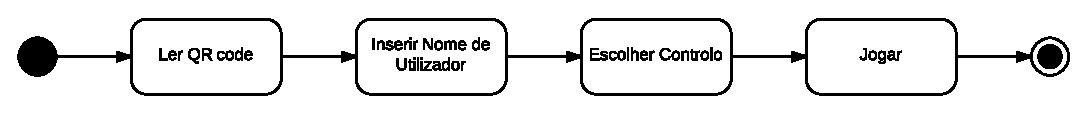
\includegraphics[width=\linewidth]{activity.pdf}
	\caption[Utilização]{Interação com a aplicação}
	\label{fig:interagir}
	\end{figure}

	Ao aproximar-se de um ecrã que tenha a correr este exemplo, o transeunte deve:

	\begin{enumerate}
		\item Ler o \textit{QR code} presente no ecrã;
		\item Introduzir um nome pelo qual quer ser identificado;
		\item Escolher o controlo desejado para jogar;
		\item Jogar.
	\end{enumerate}


	


	





